\subsubsection{La Vue}
\label{subsubsec:vue}

Chacun des deux modes de jeu possèdent une vue qui lui est propre.
Cela a été rendu possible grâce aux plusieurs classes et implémentations.

Principalement, nous avons la classe abstraite \textbf{\textit{LabyrinthView.java}} qui est étendue par la classe \textbf{\textit{LabyrinthViewImplementation.java}}.
Cette dernière possède comme attribut une instance de
\textbf{\textit{LabyrinthPanel.java}} qui est chargée de dessiner le labyrinthe à partir de cellules crées grâce à la classe \textbf{\textit{Cell.java}} qui se base sur les données du modèle.

Les labyrinthes ont un point de départ et un point d'arrivée que tous les joueurs doivent atteindre.
\subsubsection*{Le mode Classique}

La vue du mode classique (\ref{fig:ClassicModeLabyrinth} est gérée par la classe \textbf{\textit{LabyrinthClassicView.java}} qui est une extension de \textbf{\textit{LabyrintheViewImplementation.java}}).

\begin{figure}[!htb]%
    \centering
    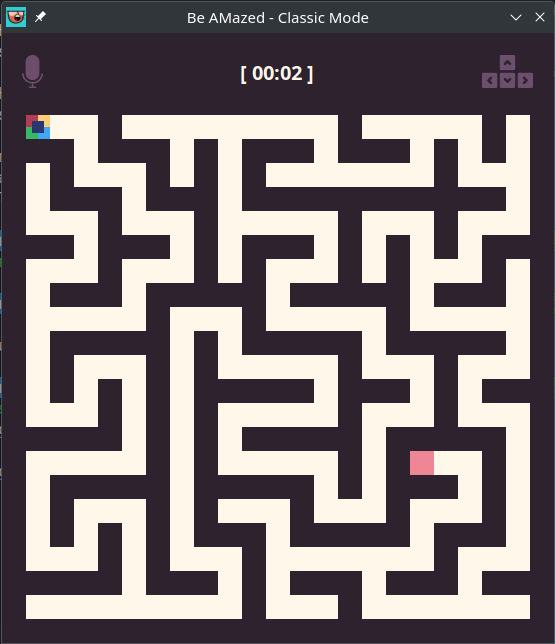
\includegraphics[width=8cm]{ressources/Implementation/Labyrinthe/Vue/Classic/Classic.png}%
    \caption{Image du mode Classique}%
    \label{fig:ClassicModeLabyrinth}
\end{figure}
\subsubsection*{Le mode Blackout}

La vue du mode Blackout (\ref{fig:BlackoutModeLabyrinth} est gérée par la classe \textbf{\textit{LabyrinthBlackoutView.java}} qui est une extension de \textbf{\textit{LabyrintheViewImplementation.java}}).

C'est un mode de jeu où les joueurs ne peuvent pas voir le labyrinthe périodiquement. Nous avons donc deux types de vues pour ce mode de jeu : une vue où le labyrinthe est visible, et une vue où le labyrinthe est caché.

Les déplacements du joueur laissent derrière lui une traînée afin de l'aider à se repérer dans le labyrinthe.

\begin{figure}[!htb]%
    \centering
    \subfloat[\centering Labyrinthe caché]{{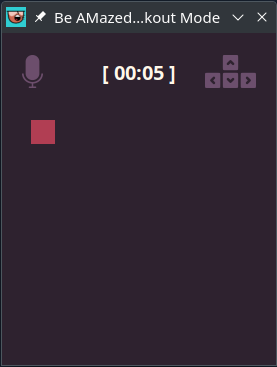
\includegraphics[width=4.4cm]{ressources/Implementation/Labyrinthe/Vue/Blackout/BlackoutDark.png}}}%
    \qquad
    \subfloat[\centering Labyrinthe visible]{{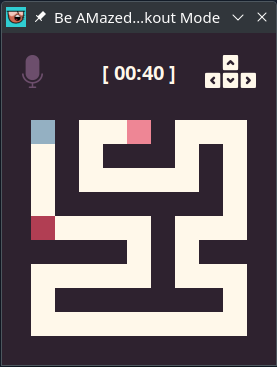
\includegraphics[width=4.4cm]{ressources/Implementation/Labyrinthe/Vue/Blackout/BlackoutLight.png}}}%
    \qquad
    \subfloat[\centering Labyrinthe caché et trainée]{{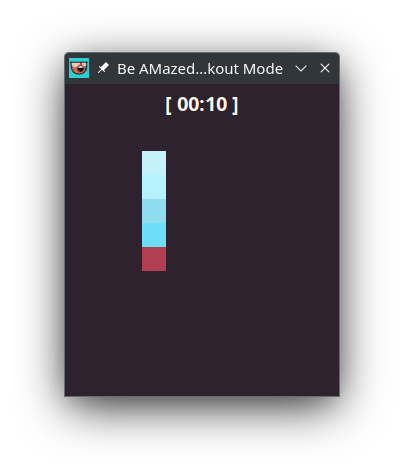
\includegraphics[width=4.4cm]{ressources/Implementation/Labyrinthe/Vue/Blackout/BlackoutDarkParticles.png}}}%
    \caption{Images du mode Blackout}%
    \label{fig:BlackoutModeLabyrinth}
\end{figure}
\FloatBarrier

\subsubsection*{Les joueurs du labyrinthe}

L'affichage des joueurs (\ref{fig:PlayersInLabyrinth} est géré par les classes \textbf{\textit{LabyrinthPanel.java}} et \textbf{\textit{Cell.java}}) en fonction de leurs positions dans le labyrinthe. Ils sont représentés par des rectangles de couleurs différentes qui changent de taille en fonction du nombre de joueurs présents sur une seule case. Nous avons choisi cette représentation car elle est simple et facile à comprendre d'un point de vue ergonomique.

\begin{figure}[!htb]
    \centering
    \subfloat[\centering 1 joueur]{{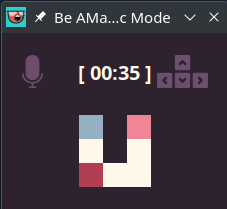
\includegraphics[width=2.3cm]{ressources/Implementation/Labyrinthe/Vue/Players/1Player.png}}}%
    \qquad
    \subfloat[\centering 2 joueurs]{{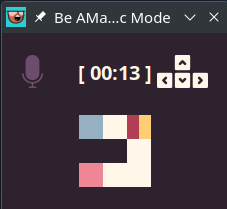
\includegraphics[width=2.3cm]{ressources/Implementation/Labyrinthe/Vue/Players/2Players.png}}}%
    \qquad
    \subfloat[\centering 3 joueurs]{{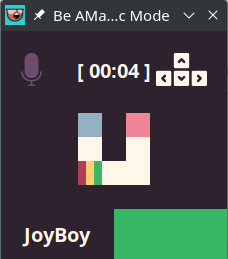
\includegraphics[width=2.3cm]{ressources/Implementation/Labyrinthe/Vue/Players/3Players.png}}}%
    \qquad
    \subfloat[\centering 4 joueurs]{{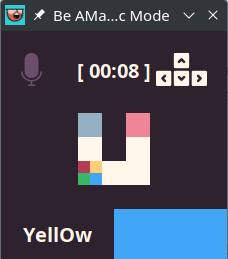
\includegraphics[width=2.3cm]{ressources/Implementation/Labyrinthe/Vue/Players/4Players.png}}}%
    \qquad
    \subfloat[\centering 5 joueurs]{{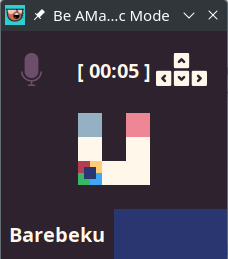
\includegraphics[width=2.3cm]{ressources/Implementation/Labyrinthe/Vue/Players/5Players.png}}}%
    \caption{Images des joueurs dans le labyrinthe}
    \label{fig:PlayersInLabyrinth}
\end{figure}
\FloatBarrier

\subsubsection*{Le décompte et le timer}

Le décompte et le timer (\ref{fig:CountdownAndTimer} sont affichés en haut au centre de chaque partie de jeu. Le décompte affiché en rouge au début de la partie permet aux joueurs de se préparer avant le début de la partie. Une fois le décompte terminé, le timer affiché en blanc commence à compter le temps écoulé depuis le début de la partie. Leurs affichage est géré par la classe \textbf{\textit{TimerPanel.java}}).

\begin{figure}[!htb]%
    \centering
    \subfloat[\centering Décompte]{{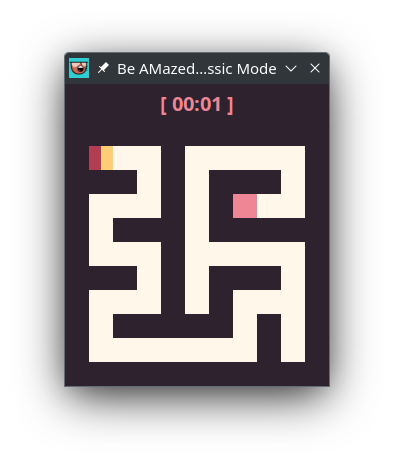
\includegraphics[width=5cm]{ressources/Implementation/Labyrinthe/Vue/CountdownTimer/CountDown.png}}}%
    \qquad
    \subfloat[\centering Timer]{{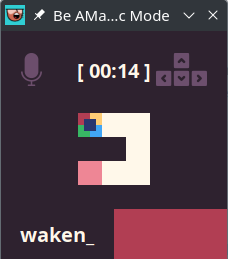
\includegraphics[width=5cm]{ressources/Implementation/Labyrinthe/Vue/CountdownTimer/Timer.png}}}%
    \caption{Images du décompte et du timer}%
    \label{fig:CountdownAndTimer}
\end{figure}
\FloatBarrier

\subsubsection*{Fin de jeu}

Lorsque la partie est terminée, une fenêtre de fin de jeu (\ref{fig:GameOverWindow} s'affiche avec le tableau des scores de chaque joueur avec des boutons en bas pour retourner au menu principal, rejouer et quitter le jeu. Cette fenêtre est gérée par la classe \textbf{\textit{GameOverPanel.java}} et \textbf{\textit{ScoreBoardPanel.java}}).

\begin{figure}[!htb]%
    \centering
    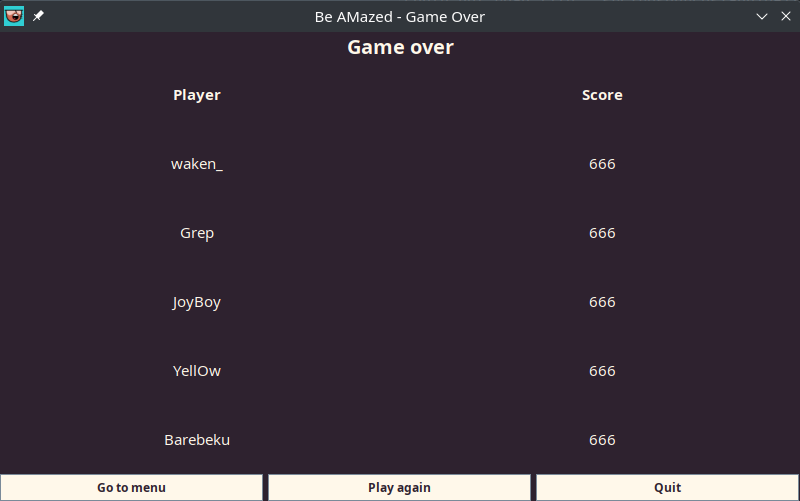
\includegraphics[width=10cm]{ressources/Implementation/Labyrinthe/Vue/GameOver.png}%
    \caption{Image de la fenêtre de fin de jeu}%
    \label{fig:GameOverWindow}
\end{figure}
\FloatBarrier

\subsubsection*{Diagramme de classe de la vue}
% TODO: Insérer une image du diagramme de classe de la vue pour les fichiers mentionnés.